\subsection{Power Measurement and Acquisition Setup}
\begin{figure}[t]
  \centering
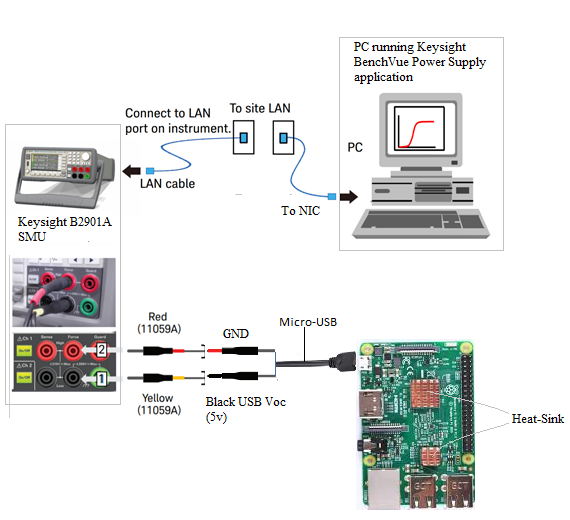
\includegraphics[width=0.9\columnwidth, height=8cm]{expsetup}
  \caption{Experimental Framework}\label{expsetup}
\end{figure}

Figure~\ref{expsetup} shows our experimental framework to measure the power and performance characteristics of the obfuscated benchmarks, and the data acquisition system. We target the Raspberry Pi (RPi) which is a popular platform for low-power and low-cost computational tasks~\cite{maksimovic2014raspberry}. Specifically, are measurements are carried out on a Raspberry Pi 3 Model B+ with a Broadcom BCM2837B0 SoC. This is a quad-core A53 (ARMv8) 64-bit 1.4GHz processor with 1GB LPDDR2 SDRAM. It rons on 5V/2.5A DC input power via a microUSB connector. Its operating temperature is between 0 to $60^{\circ}C$.

We have built a custom setup to measure the power consumption from the RPi. We power the RPi via a microUSB from a stable 5V/2.5A power supply. (see Figure~\ref{expsetup}), from which the power consumed by the RPi is $P$ = $V\times I$.
To provide the required power supply to the RPi and capture the power drawn during code execution, we  use the Keysight SMU source meter unit. We use a 2-wire connection with SMU Kelvin probes to an open-ended microUSB 2-wire cable which in turn powers the Raspberry Pi with constant and accurate power supply. The SMU is connected to a PC via a LAN cable. This is used to control the SMU via Keysight commands to extract the required current and voltage values from the SMU loaded into the Keysight BenchVue Power Supply PC application.

The RPi has an on-chip temperature sensor which measures the temperature of the CPU. This provides additional information of the heat state of the RPi. We used 2 heat-sinks and an external cooling fan in an air conditioned environment to maintain optimal working conditions for the Pi.  

The obfuscated target programs are executed on the RPi and power samples are acquired on the PC. Each experiment is executed 5 times, and execution times and power values are averaged over the runs.